Korzystając z~wiedzy i~doświadczeń wyniesionych z~sekcji~\ref{sec:przeglad} niniejszego sprawozdania, zdecydowaliśmy się na stworzenie systemu odpowiadającego na pytania ogólne, z~wyszczególnieniem pytań o~fakty dotyczące:
\begin{itemize}
    \item osób,
    \item miejsc,
    \item dat,
    \item cech wielkościowych,
    \item przedmiotów.
\end{itemize}

Bazą więdzy systemu będzie sieć WWW. Do wyszukiwania dokumentów w~sieci~WWW, wykorzystane zostaną wyszukiwarki internetowe: \emph{Google\footnote{www.google.pl}}, \emph{Bing\footnote{www.bing.com}}, \emph{Yahoo\footnote{www.search.yahoo.com}} oraz \emph{DuckDuckGo\footnote{duckduckgo.com}}. Podobnie jak we wcześniej omawianym systemie AskMSR~\cite{brill2002analysis}, do dalszej analizy przekazywane będą jedynie \emph{snippety}, co pozwoli na uproszczenie etapu filtracji akapitów.

Odpowiedzią na przedstawione pytanie, będzie prosta odpowiedź typu \emph{Named-Enitity}. Nie przewidujemy odpowiadania na pytania w~języku naturalnym.

\subsection{Zarys algorytmu}
Na rysunku~\ref{fig:algorithm-overview}, przedstawiony został ogólny schemat algorytmu odpowiadania na pytania.

\begin{figure}[h]
    \centering
    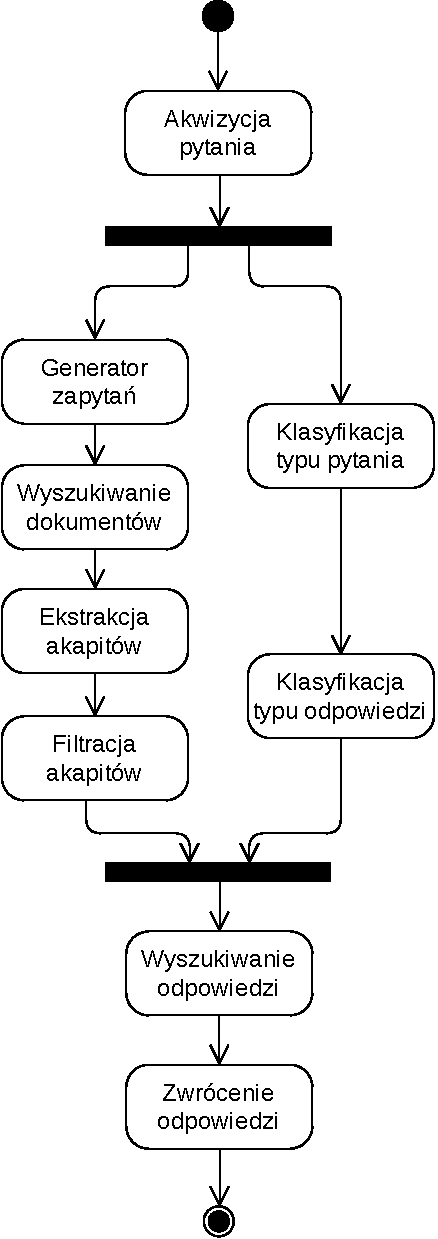
\includegraphics[width=0.7\columnwidth]{figures/WEDT-Algorytm.pdf}
    \caption{Ogólny schemat algorytmu odpowiadania na pytania}
    \label{fig:algorithm-overview}
\end{figure}

Pierwszym krokiem algorytmu jest akwizycja pytania od użytkownika systemu. Każde pytanie będzie analizowane w~sposób indywidualny, bez przechowywania wcześniejszych pytań i~utrzymywania kontekstu. Nie zakładamy również żadnego profilowania użytkowników, ponieważ typowo proste pytania o~fakty, są ze sobą słabo powiązane.

W~kolejnym kroku, strumień sterowania rozdwaja się i~jest przekazywany do dwóch modułów, które przetwarzają zapytanie równolegle. Moduł akwizycji wiedzy, na podstawie przekazanego pytania, stara się uzyskać jak największą ilość \emph{snippetów}, generując specjalistyczne zapytania do każdej z~czterech wyszukiwarek, tak jak to zostało przedstawione w~\cite{zheng2002answerbus}. Oprócz tego, aby wykorzystać redundantość sieci~WWW, do wyszukiwarek wysłane zostaną również okrojone zapytania, pozbawione części słów, tak aby zwiększyć zakres poszukiwań, podobnie jak w~\cite{brill2002analysis}. Aby zwiększyć rozmiar zbioru wyszukanych \emph{snippetów}, słowa kluczowe w~zapytaniu, będą wymieniane na ich synonimy~\cite{przybyla-2013-question}.

W~trakcie wyszukiwania \emph{snippetów}, w~drugiej gałęzi algorytmu, następuję klasyfikacja typu pytania i~oczekiwanej odpowiedzi. Klasy pytań są definiowane przez zaimki pytające, podobnie jak w~\cite{gupta2012survey}. Wyróżniamy pytania typu: \emph{Kto?}, \emph{Jaki/Jaka/Jakie?}, \emph{Jak?}, \emph{Gdzie?}, \emph{Kiedy?}, \emph{Co?} oraz \emph{Który/Która/Które?}. Wykrywanie typu pytania odbywać się będzie w~prosty sposób, stosując reguły podstawieniowe oraz rozkład zdania. Określanie typu oczekiwanej odpowiedzi będzie wynikało głównie z~typu pytania, wspartej możliwością odpytania usługi \emph{plWordNet}~\cite{MazPiaRudSzpaKedz:16} oraz dodatkowym sprawdzeniem wyrażeń regularnych.

Każdy wyszukany \emph{snippet} zostanie poddany analizie morfologicznej, po której przyporządkowana zostanie mu odpowiednia ocena. W~każdym zdaniu, za pomocą taggera oraz \emph{plWordNetu} wyszukiwane będą \emph{Named-Entities}, które mogą stanowić potencjalną odpowiedź na pytanie. Ostatnim krokiem procesu będzie zwrócenie najlepszej odpowiedzi lub zbioru najlepszych odpowiedzi. Do odpowiedzi dołączony może zostać link ze źródłem, w~celu umożliwienia użytkownikowi systemu osobistej weryfikacji odpowiedzi.

\subsection{Dekompozycja systemu}
Zaprojektowany system składa się z~kilku funkcjonalnych komponentów, z~czego tylko część zostanie przez nas zrealizowana w~całości. Duży fragment systemu będzie wykorzystywał gotowe komponenty takie jak \emph{plWordNet} czy wyszukiwarki internetowe. Na rysunku \ref{fig:system-components} przedstawiony został podział na komponenty funkcjonalne, ze szczególnym wyróżnieniem relacji pomiędzy nimi.

\begin{figure}[h]
    \centering
    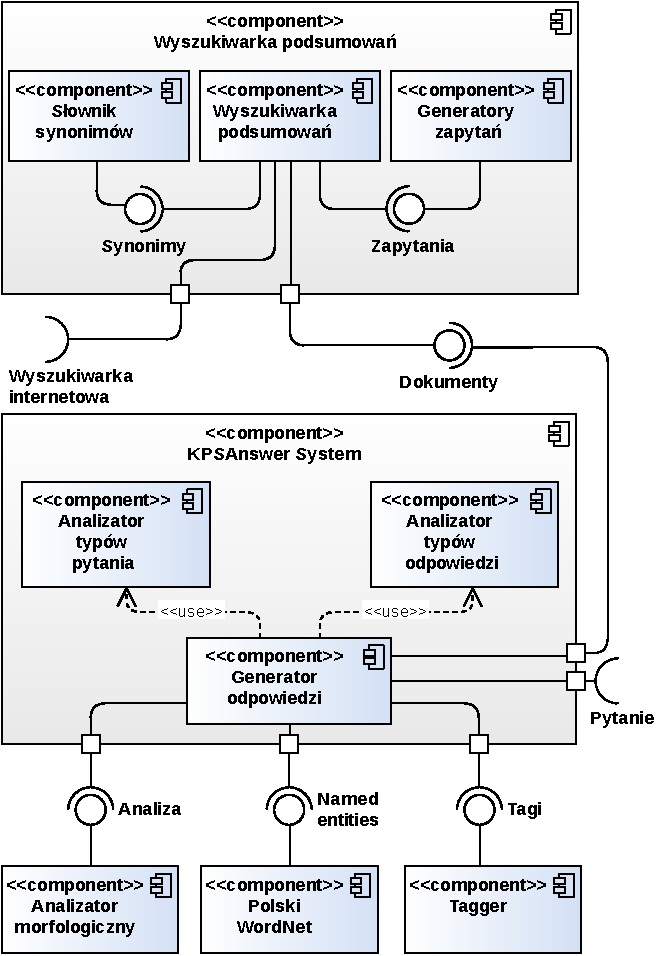
\includegraphics[width=\columnwidth]{figures/WEDT-Komponenty.pdf}
    \caption{Podział systemu KPSAnswer na funkcjonalne komponenty}
    \label{fig:system-components}
\end{figure}

Planowany podział zakłada istnienie dwóch, głównych komponentów:
\emph{KPSAnswer System\footnote{Nazwa KPS pochodzi od pierwszych liter nazwisk autorów}} oraz wyszukiwarki podsumowań, wspieranych kilkoma komponentami pobocznymi.
Komponent \emph{KPSAnswer System} zajmuje się generacją odpowiedzi na pytania przychodzące z~zewnątrz, korzystając z~interfejsu \texttt{Pytania}. W~celu wygenerowania odpowiedzi, komponent ten odpytuje \texttt{Wyszukiwarkę podsumowań} przy użyciu interfejsu \texttt{Dokumenty} o~zbiór podsumowań, mogących zawierać odpowiedź. \texttt{Wyszukiwarka podsumowań} zdobywa podsumowania odpytując strony implementujące interfejs \texttt{Wyszukiwarka internetowa}.

\subsection{Propozycja implementacji}
Wydzielenie dwóch głównych komponentów, komunikujących się z~komponentami pobocznymi za pomocą interfejsów komunikujących, pozwala na wydzielenie bytów, aplikacji w~systemie. Proponowany przez nas podział na aplikacje, przedstawiony został na rysunku~\ref{fig:system-deployment}.

\begin{figure}[h!]
    \centering
    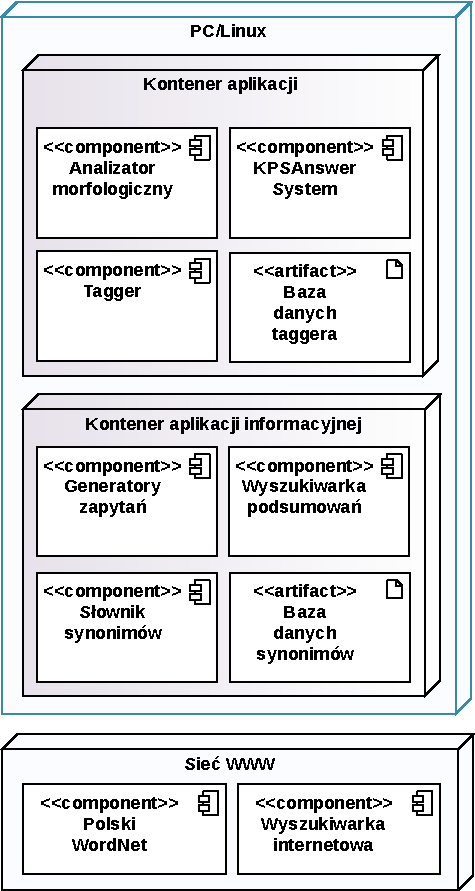
\includegraphics[width=0.8\columnwidth]{figures/WEDT-Deployment.pdf}
    \caption{Diagram rozmieszczenia systemu KPSAnswer}
    \label{fig:system-deployment}
\end{figure}

Na maszynie PC z~systemem operacyjnym Linux uruchomione zostaną dwa procesy, które przygotwane zostaną przy użyciu języka wysokiego poziomu Python w~wersji~3. Pierwszy z~nich będzie przyjmował pytania za pomocą wystawionego interfejsu REST API. Dzięki temu, aplikacja będzie mogła być odpytywana za pomocą wiersza poleceń, programów typu Postman lub dedykowanego interfejsu graficznego. Drugi proces odpowiedzialny będzie za przeszukiwanie sieci WWW, generację odpowiednich zapytań oraz odpytywanie wyszukiwarek i~agregację podsumowań. Obie aplikacje będą komunikowały się z~aplikacjami w~sieci WWW, dlatego też maszyna będzie musiała być cały czas podłączona do internetu. Zastosowanie komunikacji z~użyciem protokołu HTTP pozwoli na potencjalne uruchomienie systemu w~chmurze, tak jak system Watson, omawiany w~\cite{lapshin2012question}.